\documentclass[12pt]{article}

\usepackage{sbc-template}

\usepackage{graphicx,url}

\usepackage[brazil]{babel}   
\usepackage[latin1]{inputenc}  

     
\sloppy

\title{Estruturas de dados eficientes\\ para algoritmo gen\'{e}tico}

\author{Raphael R. Gon\c{c}alves\inst{1}}


\address{Instituto de Computa\c{c}\~{a}o -- Universidade Federal Fluminense
  (UFF)\\
  24.210-346 -- Niter\'{o}i -- RJ -- Brasil
}

\begin{document} 

\maketitle

\begin{abstract}
    TODO
\end{abstract}
     
\begin{resumo} 
    A FAZER
\end{resumo}


\section{Introdu\c{c}\~{a}o}

TODO

\section{Revis\~{a}o da Literatura} \label{sec:firstpage}

TODO

\section{O Algoritmo Gen\'{e}tico}

TODO

\section{Desafios durante a implementa\c{c}\~{a}o}

TODO

\subsection{Rota\c{c}\~{a}o de vetores}

A rota\c{c}\~{a}o de vetores \'{e} uma opera\c{c}\~{a}o aplicada em \textit{arrays} e outros
\textit{containers} utilizada diferentes casos de uso na computa\c{c}\~{a}o.
Ela consiste em retirar um elemento de uma das extremidades do vetor e
inser\'{i}-lo na outra extremidade, causando a movimenta\c{c}\~{a}o de todos os elementos
para a esquerda ou para a direita, dependendo de qual a extremidade que o elemento
foi removido.

Dentro do contexto de algoritmos gen\'{e}ticos, para realizar um \textit{crossover} pode ser
necess\'{a}rio realizar diferentes opera\c{c}\~{o}es em um vetor, e uma delas que \'{e} muito
utilizada \'{e} a rota\c{c}\~{a}o. Um dos operadores de \textit{crossover} que requer uma
rota\c{c}\~{a}o \'{e} o \textit{Order Crossover} (OX), onde \'{e} selecionado um subconjunto dos genes
de um indiv\'{i}duo e inserido em outro indiv\'{i}duo, causando uma rota\c{c}\~{a}o dos elementos j\'{a}
inseridos no segundo indiv\'{i}duo tanto para a direita quanto para a esquerda. Este comportamento \'{e}
ilustrado na Figura~\ref{fig:orderCrossover}

\begin{figure}[ht]
\centering
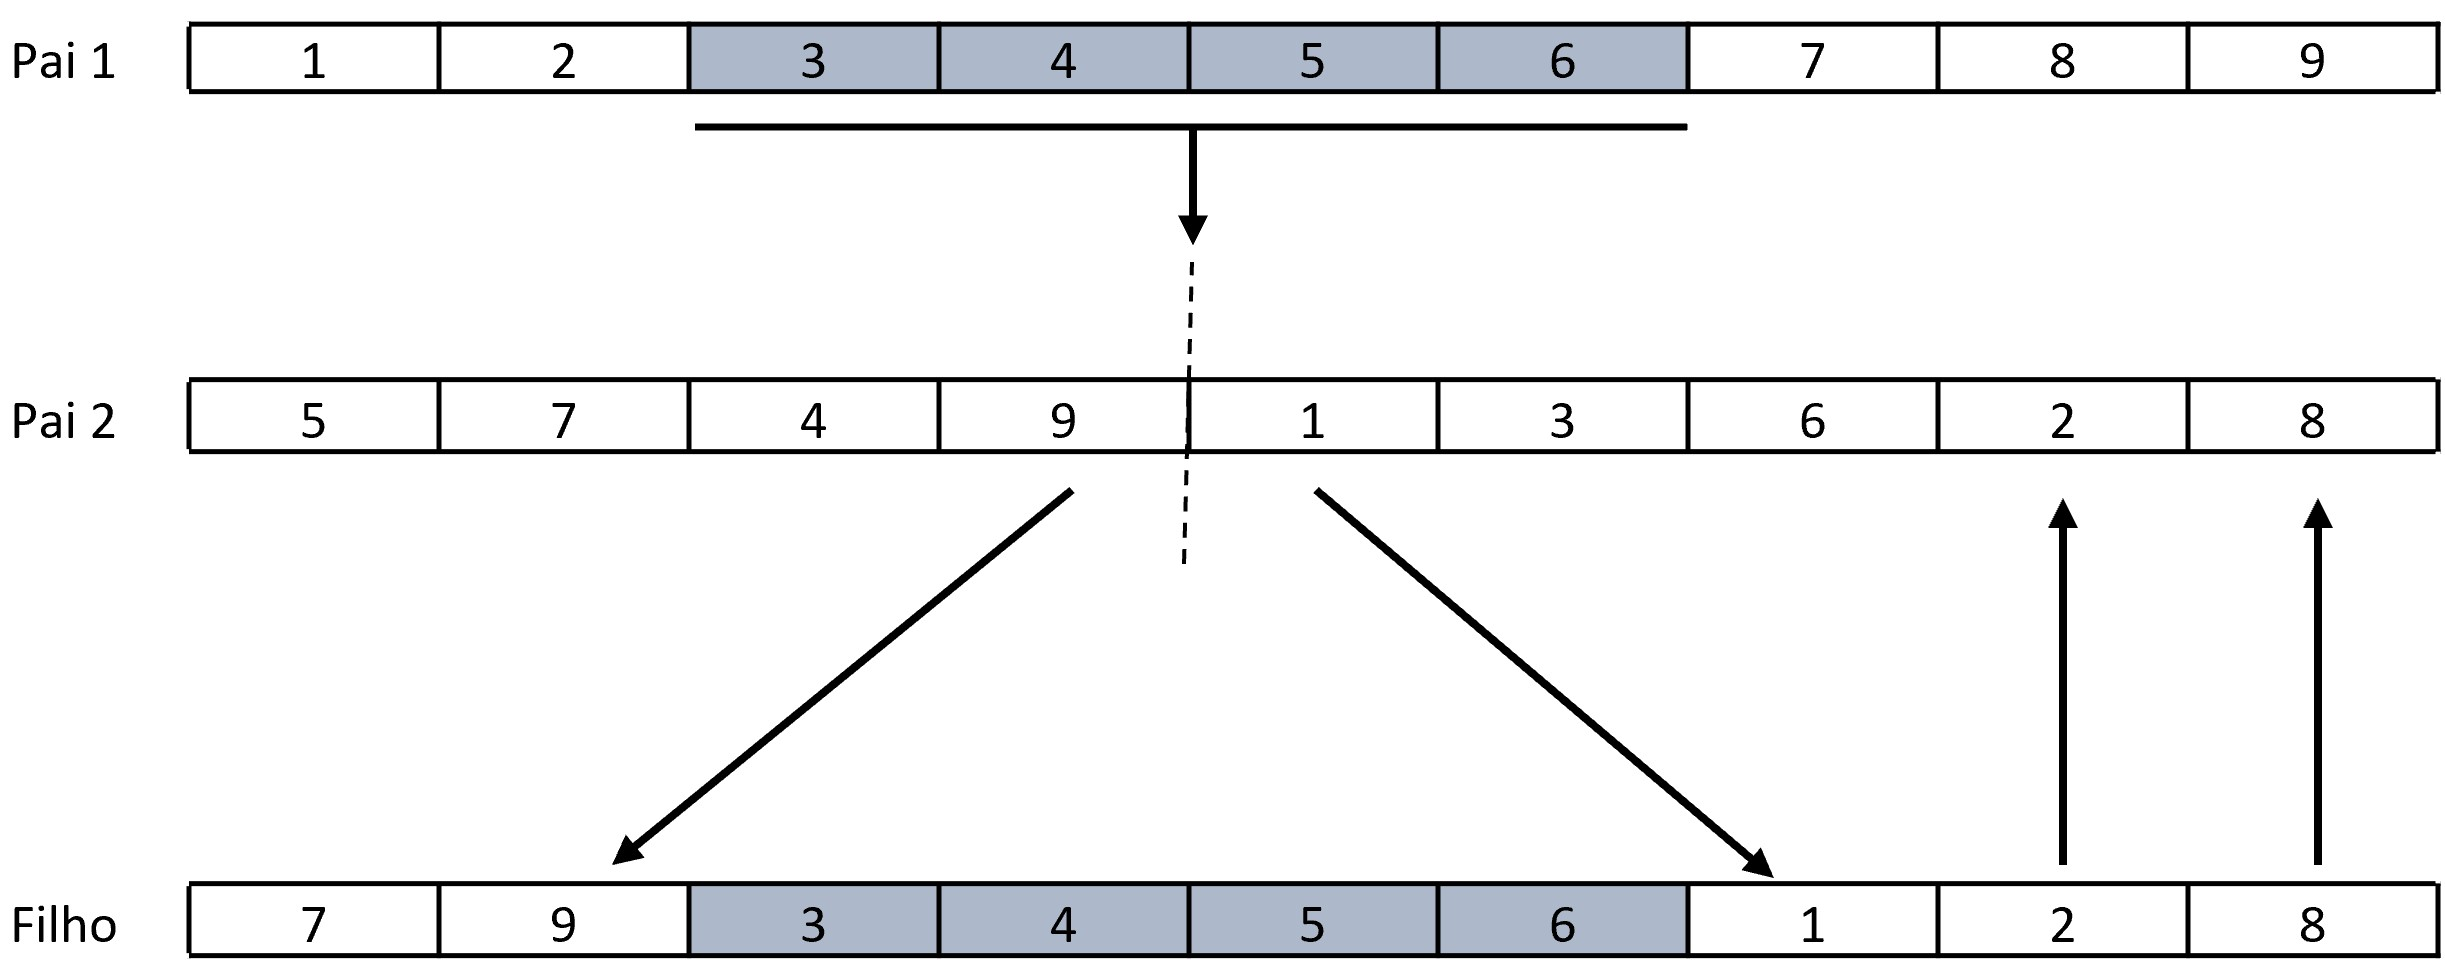
\includegraphics[width=.8\textwidth]{order_crossover.jpg}
\caption{O funcionamento do Order Crossover}
\label{fig:orderCrossover}
\end{figure}

Dependendo da estrutura de dados e o algoritmo utilizado, uma rota\c{c}\~{a}o pode levar \`{a}
copia de todos os elementos de um \textit{container} para outro, tendo em vista que, por exemplo,
um vetor somente permite a inser\c{c}\~{a}o de elementos em somente uma extremidade. Este
comportamento pode tornar esta simples tarefa uma, rotina de complexidade $\mathcal{O}(n)$.

Entretanto esta complexidade pode ser reduzida simplesmente utilizando uma estrutura do tipo
\textit{Deque} (\textit{Dual-Ended Queue}). Esta estrutura de dados permite que sejam inseridos
elementos por ambos os lados, permitindo a rota\c{c}\~{a}o dos elementos com complexidade
$\mathcal{O}(n)$ com f\'{a}cil implementa\c{c}\~{a}o.

\subsection{Gera\c{c}\~{a}o aleat\'{o}ria de elementos n\~{a}o repetitivos}

Ao inicializar uma popula\c{c}\~{a}o de indivíduos aleatoriamente, em muitos casos existe
a necessidade de um indivíduo não possuir genes com valores repetidos.

\subsection{Gera\c{c}\~{a}o alet\'{o}ria de subvetores}

TODO

\section{Implement\c{c}\~{a}o}

TODO

\section{Conclus\c{c}\~{a}o}

TODO

\section{Figures and Captions}\label{sec:figs}


Figure and table captions should be centered if less than one line
(Figure~\ref{fig:exampleFig1}), otherwise justified and indented by 0.8cm on
both margins, as shown in Figure~\ref{fig:exampleFig2}. The caption font must
be Helvetica, 10 point, boldface, with 6 points of space before and after each
caption.

\begin{figure}[ht]
\centering
\includegraphics[width=.5\textwidth]{fig1.jpg}
\caption{A typical figure}
\label{fig:exampleFig1}
\end{figure}

\begin{figure}[ht]
\centering
\includegraphics[width=.3\textwidth]{fig2.jpg}
\caption{This figure is an example of a figure caption taking more than one
  line and justified considering margins mentioned in Section~\ref{sec:figs}.}
\label{fig:exampleFig2}
\end{figure}

In tables, try to avoid the use of colored or shaded backgrounds, and avoid
thick, doubled, or unnecessary framing lines. When reporting empirical data,
do not use more decimal digits than warranted by their precision and
reproducibility. Table caption must be placed before the table (see Table 1)
and the font used must also be Helvetica, 10 point, boldface, with 6 points of
space before and after each caption.

\begin{table}[ht]
\centering
\caption{Variables to be considered on the evaluation of interaction
  techniques}
\label{tab:exTable1}
\includegraphics[width=.7\textwidth]{table.jpg}
\end{table}

\section{Images}

All images and illustrations should be in black-and-white, or gray tones,
excepting for the papers that will be electronically available (on CD-ROMs,
internet, etc.). The image resolution on paper should be about 600 dpi for
black-and-white images, and 150-300 dpi for grayscale images.  Do not include
images with excessive resolution, as they may take hours to print, without any
visible difference in the result. 

\section{References}

Bibliographic references must be unambiguous and uniform.  We recommend giving
the author names references in brackets, e.g. \cite{knuth:84},
\cite{boulic:91}, and \cite{smith:99}.

The references must be listed using 12 point font size, with 6 points of space
before each reference. The first line of each reference should not be
indented, while the subsequent should be indented by 0.5 cm.

\bibliographystyle{sbc}
\bibliography{sbc-template}

\end{document}
